\documentclass{article}
\usepackage[polish]{babel}
\usepackage{polski}
\selecthyphenation{polish}
\usepackage[utf8]{inputenc}

\usepackage{algorithm}
\usepackage{algpseudocode}
\usepackage{chngpage}
\usepackage[colorlinks, urlcolor=blue]{hyperref}
\usepackage{epsf}
\usepackage{etaremune}
\usepackage[pdftex, dvips]{graphicx}
\usepackage{multirow}
\usepackage[parfill]{parskip}
\usepackage{url}

\algnewcommand\And{\,\textbf{and}\,}
\algnewcommand\Or{\,\textbf{or}\,}


\title {PAN 2014 Author Profiler - podręcznik użytkownika}

\author{Jacek Kowalski, Paweł Lipski}

\begin{document}
\maketitle

\section{Pobieranie kodu}

\texttt{git clone \href{https://github.com/tilius/author-profiler.git}{https://github.com/tilius/author-profiler.git}}

Kod był uruchamiany pod wersją 2.7.3 Pythona.

\section{Instalacja bibliotek obliczeniowych}

\subsection{LIBLINEAR}

Bibliotekę można pobrać z \href{http://www.csie.ntu.edu.tw/~cjlin/liblinear/}{http://www.csie.ntu.edu.tw/~cjlin/liblinear/} (sekcja Download LIBLINEAR).

Po rozpakowaniu wystarczy wydać polecenie make. Powstały plik wykonywalne train oraz predict należy umieścić np. w /usr/local/bin (tak, aby były one dostępne przez PATH) pod następującym nazwami:
\begin{itemize}
\item train $\rightarrow$ linear-train
\item predict $\rightarrow$ linear-predict
\end{itemize}

\subsection{LIBSVM}

Domyślnie aplikacja wykorzystuje LIBLINEAR. Użycie LIBSVM do obliczeń można wymusić poprzez przekazanie opcji \texttt{--libsvm} do polecenia train.py.

Bibliotekę można pobrać z \href{http://www.csie.ntu.edu.tw/~cjlin/libsvm/}{http://www.csie.ntu.edu.tw/$\sim$cjlin/libsvm/} (sekcja Download LIBSVM).

Po rozpakowaniu wystarczy wydać polecenie make, a następnie umieścić trzy pliki wykonywalne (svm-train, svm-scale oraz svm-predict) np. w /usr/local/bin (tak, aby były one dostępne przez PATH).


\section{Instalacja NTLK}

Zgodnie z \href{http://www.nltk.org/install.html}{http://www.nltk.org/install.html}, zakładając, że w systemie jest dostępny pip, należy uruchomić z shella:

\texttt{sudo pip install -U numpy \\
sudo pip install -U pyyaml nltk}

Następnie należy ściągnąć dane NTLK (dokładniej Part Of Speech Tagger). Po wejściu w interaktywną powłokę Pythona należy wpisać:

\texttt{import nltk \\
nltk.download("maxent\_treebank\_pos\_tagger")}


\section{Uruchamianie}

\subsection{Trenowanie}

\texttt{train.py [-h] -i corpus\_dir -o model\_dir [--disjoint] [--libsvm]}

Zakłada się, że \texttt{corpus\_dir} jest katalogiem, w którym znajdują się pliki XML zgodne z formatem przewidzianym dla PAN 2014. Uprzednio utworzone przez train.py pliki w \texttt{model\_dir} zostaną nadpisane. \\
Niestandardowa opcja \texttt{--disjoint} uruchamia trenowanie w trybie osobnego trenowania i klasyfikacji dla płci oraz wieku. Odpowiedni obiekt klasyfikatora wraz z wszystkimi niezbędnymi rezultatami zostanie w takim przypadku zapisany do folderu \texttt{model\_dir}. Z tego względu nie przekazuje się tej opcji do \texttt{classify.py}. \\
Niestandardowa opcja \texttt{--libsvm} wykorzystuje bibliotekę LIBSVM (zamiast domyślnej LIBLINEAR). Również tutaj nie ma potrzeby przekazywania tej opcji do \texttt{classify.py} - informacja o bibliotece zostanie zaszyta w plikach modelu.

\subsection{Klasyfikacja}

\texttt{classify.py [-h] -i corpus\_dir -m model\_dir -o output\_dir  [--truth truth\_file] [--accuracy accuracy\_output\_file]}

Zakłada się, że \texttt{corpus\_dir} jest katalogiem, w którym znajdują się pliki XML zgodne z formatem przewidzianym dla PAN 2014. Uprzednio utworzone przez classify.py pliki w \texttt{output\_dir} zostaną nadpisane. \\
Niestandardowa (i nieobowiązkowa) opcja \texttt{--truth truth\_file} wskazuje plik zawierający faktyczne wyniki klasyfikacji - przyjmujemy format zgodny z tym używany w plikach PAN2013. Taki plik można też wygenerować za pomocą skryptu scripts/make-truth.sh, podając w parametrze katalog - wynik zostanie zapisany do pliku truth.dat w tym katalogu.
Niestandardowa (i nieobowiązkowa) opcja \texttt{--accuracy accuracy\_output\_file} wskazuje plik, do którego zostanie zapisana linia z informacją o trafności klasyfikacji (używane w skryptach).


\section{Wyniki}

Wszystkie testy były uruchamiane na Ubuntu 12.04 wirtualizowanym w VMware Player na Windows 7, na procesorze i7 przy włączonym VT-X. \\

\begin{description}

\item[Styl] rodzaj danych (fragment korpusu treningowego PAN14), na jakich uruchamiane były testy \\

\item[$N_{total}$] całkowity rozmiar danego fragmentu PAN14
\item[$N_{train}, N_{test}$] rozmiar korpusu treningowego i testowego, wydzielonych z wybranego fragmentu PAN14
\item[$N_{maj}$] rozmiar klasy większościowej w obrębie korpusu testowego \\

\item[linear] użyto biblioteki LIBLINEAR
\item[svm] użyto biblioteki LIBSVM
\item[joint] trenowanie i klasyfikacja były przeprowadzane dla klas będących kombinacją płci i wieku
\item[disjoint] trenowanie i klasyfikacja były przeprowadzane oddzielnie dla płci i wieku \\

\end{description}


\begin{adjustwidth}{-3.5cm}{-0cm}

\begin{tabular}{|p{2cm}|p{2cm}|p{2cm}|p{2cm}|p{3cm}|p{3cm}|p{3cm}|}

\hline

\textbf{Styl} & \textbf{$N_{total}$} & \textbf{$N_{train}, N_{test}$} & $N_{maj}$ & \textbf{Konfiguracja} & \textbf{Dokładność} & \textbf{Czas} \\  \hline

\multirow{4}{*}{Blog} & \multirow{4}{*}{147}	& \multirow{4}{*}{75} & \multirow{4}{*}{17} & 
linear, joint & 28.00\% (21/75) & 1677 sec \\  \cline{5-7}
& & & & 
linear, disjoint & 26.67\% (20/75) & 2833 sec \\  \cline{5-7}
& & & & 
svm, joint & 16.00\% (12/75) & 1695 sec \\  \cline{5-7}
& & & & 
svm, disjoint & 16.00\% (12/75) & 2711 sec \\  \hline

\multirow{12}{*}{Reviews} & \multirow{12}{*}{4470} & \multirow{4}{*}{200} & \multirow{4}{*}{39} & 
linear, joint & 16.00\% (32/200) & 316 sec \\  \cline{5-7}
& & & & 
linear, disjoint & 12.00\% (24/200) & 544 sec \\  \cline{5-7}
& & & & 
svm, joint & 12.50\% (25/200) & 319 sec \\  \cline{5-7}
& & & & 
svm, disjoint & 11.50\% (23/200) & 543 sec \\  \cline{3-7}

& & \multirow{4}{*}{1000} & \multirow{4}{*}{133} & 
linear, joint & 28.30\% (283/1000) & 1590 sec \\  \cline{5-7}
& & & & 
linear, disjoint & 28.90\% (289/1000) & 2895 sec \\  \cline{5-7}
& & & & 
svm, joint & 13.30\% (133/1000) & 1683 sec \\  \cline{5-7}
& & & & 
svm, disjoint & 13.30\% (133/1000) & 2912 sec \\  \cline{3-7}

& & \multirow{4}{*}{2000} & \multirow{4}{*}{261} & 
linear, joint & 36.60\% (732/2000) & 3565 sec \\  \cline{5-7}
& & & & 
linear, disjoint & 34.05\% (681/2000) & 6212 sec \\  \cline{5-7}
& & & & 
svm, joint & \textit{(skipped)} & N/A \\  \cline{5-7}
& & & & 
svm, disjoint & \textit{(skipped)} & N/A \\  \hline

\multirow{4}{*}{Social media} & \multirow{4}{*}{7746} & \multirow{4}{*}{150} & \multirow{4}{*}{39} & 
linear, joint & 58.67\% (88/150) & 1536  sec \\  \cline{5-7}
& & & & 
linear, disjoint & 56.00\% (84/150) & 2622 sec \\  \cline{5-7}
& & & & 
svm, joint & 26.00\% (39/150) & 3257 sec \\  \cline{5-7}
& & & & 
svm, disjoint & 25.33\% (38/150) & 5646 sec \\  \hline


\end{tabular}

\end{adjustwidth}

\section{Wnioski}

Użycie LIBLINEAR przynosiło zdecydowanie lepsze rezulataty niż użycie LIBSVM. Ta druga w niektórych przypadkach zwracała dla wszystkich klasyfikowanych obiektów klasę większościową, a w jeszcze innych jej dokładność była nawet mniejsza niż naiwnej klasyfikacji wg klasy większościowej.

Nie miało większego znaczenia dla dokładności, czy trenowanie i klasyfikacja były przeprowadzane dla klas będących kombinacją płci i wieku, czy oddzielnie dla płci i wieku. W tym drugim przypadku jednak znacznie więcej czasu pochłaniały obliczenia, które przeprowadzać trzeba było dla obu wielkości oddzielnie.

Zdecydowanie największą część czasu zajmowały obliczenia (tagowanie części mowy) wykonywane przez NTLK.

\textbf{TODO - coś o tym, co się udało}

\section{Wykresy}

\begin{figure}[h]
\centering
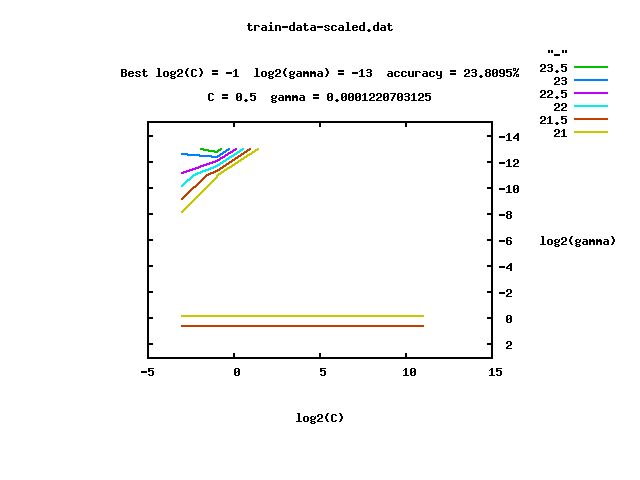
\includegraphics[scale=1.0]{logc_loggamma_acc}\label{fig:chart}
\caption{Wykres zależności dokładności od parametrów $C$ oraz $\gamma$}
\end{figure}

\end{document} 
